\documentclass[11pt,a4paper]{article}

% --- Packages ---
\usepackage[utf8]{inputenc}
\usepackage[T1]{fontenc}
\usepackage[english]{babel}
\usepackage{amsmath,amssymb,amsfonts,amsthm}
\usepackage{geometry}
\geometry{margin=1in}
\usepackage{graphicx}
\usepackage{hyperref}
\usepackage{xcolor}
\usepackage{cite}
\usepackage{booktabs}
\usepackage{microtype}
\usepackage{physics}
\usepackage{tikz}
\usetikzlibrary{babel,arrows.meta,decorations.pathmorphing}

\hypersetup{
    pdftitle={The Strong Nuclear Force, Vacuum Saturation, and the Geometry of Quark Confinement: 1D Flux Tubes and the Cornell Potential},
    pdfauthor={Muhammed Furkan Haydari},
    pdfsubject={Nuclear Physics, Quantum Chromodynamics, Quark Confinement, Flux Tube},
    pdfkeywords={Strong Force, Quark Confinement, Vacuum Saturation, 1D Flux Tube, Cornell Potential, Regge Trajectories},
    colorlinks=true,
    linkcolor=blue!70!black,
    citecolor=red!70!black,
    urlcolor=blue!80!black
}

% --- Theorem Environments ---
\newtheorem{theorem}{Theorem}[section]
\newtheorem{definition}{Definition}[section]
\newtheorem{axiom}{Aksiyom}[section]
\newtheorem{corollary}{Corollary}[theorem]
\newtheorem{lemma}[theorem]{Lemma}
\newtheorem{remark}{Remark}[section]

\title{\textbf{The Strong Nuclear Force, Vacuum Saturation, and the Geometry of Quark Confinement: \\ 1D Flux Tubes and the Cornell Potential}}

\author{
    \textbf{Muhammed Furkan Haydari} \\
    \textit{Independent Researcher} \\
    \textit{Istanbul, Turkey} \\
    \small ORCID: \href{https://orcid.org/0009-0003-2854-3947}{0009-0003-2854-3947}
}

\date{\today}

\begin{document}

\maketitle

\begin{abstract}
    In this paper, we model hadronic bound states and non-perturbative strong nuclear interactions within the framework of Scale-Time Calculus and effective flux tube geometry. In the Standard Model, Quantum Chromodynamics (QCD) and $SU(3)_c$ color gauge symmetry describe quark interactions, where lattice QCD computations confirm a linear confining potential ($V(r) \propto \sigma r$) at hadronic distances ($r \gtrsim 0.5\text{ fm}$). Here, we investigate this confining regime as an effective geometric transition where field lines collapse into a collimated 1-dimensional cylindrical vortex tube (\textit{flux tube}) bridging the quarks.

    While macroscopic gravitational and atomic electromagnetic fields spread across 3-dimensional spherical shells ($1/r^2$), at femtometer scales ($r \sim 10^{-15}\text{ m}$) the intense concentration of color-field lines leads to flux collimation with constant cross-sectional area. Because the effective cross-sectional area remains locked at the hadronic scale, the effective tension along the tube is distance-independent ($\sigma \approx 1\text{ GeV/fm} \approx 1.6 \times 10^5\text{ N}$), analytically yielding the Cornell confining potential. Meson Regge trajectories ($J \propto M^2$) emerge directly from the relativistic rotation of the flux tube, while the overlap of contraction basins at $r \to 0$ naturally accounts for asymptotic freedom.
\end{abstract}

\vspace{1em}
\noindent\textbf{Keywords:} Strong Nuclear Force, Scale-Time Calculus, Vacuum Saturation, Quark Confinement, Regge Trajectories, Asymptotic Freedom, Flux Tube.

\vspace{1em}
\hrule
\vspace{0.8em}
\tableofcontents
\vspace{0.8em}
\hrule
\vspace{1.5em}

\section{Introduction and Non-Perturbative QCD Phenomenology}
\label{sec:giris}

In modern hadronic physics, the strong interaction is formulated as the gauge coupling between quarks and $SU(3)_c$ color gauge bosons (gluons). This dynamics exhibits two distinct regimes:
\begin{enumerate}
    \item \textbf{Asymptotic Freedom:} At ultra-short distances ($r \to 0$ or $Q^2 \to \infty$), the running coupling constant decreases logarithmically, and quarks behave as quasi-free particles~\cite{gross1973,politzer1973}.
    \item \textbf{Quark Confinement:} As quarks are separated, the effective color-electric string tension remains constant ($\sigma \approx 1\text{ GeV/fm}$), preventing isolated free color charges from being observed.
\end{enumerate}

While perturbative QCD provides exact analytical solutions at high energies, the non-perturbative confining regime in the infrared is typically investigated via lattice QCD simulations. In Scale-Time Calculus~\cite{scale_calculus}, this confining regime is modeled geometrically as a \textbf{dimensional crossover from 3D spherical dilution to a 1D collimated flux tube}.

\section{The Effective 1D Flux Tube Geometry and String Tension}
\label{sec:doyum_mekanizmasi}

In the gravitational and electromagnetic regimes, field lines directed toward a bound center spread across 3-dimensional spherical shells ($A(r) = 4\pi r^2$), and the flux density decays as $1/r^2$.

However, at femtometer scales ($r \sim 10^{-15}\text{ m}$), the non-Abelian self-interaction of color gluons (or in dual superconductor models, the dual Meissner effect) prevents $1/r^2$ spherical dilution. The dynamical field between two quarks is compressed into a \textbf{1-dimensional cylindrical vortex tube (\textit{flux tube} / effective string)} whose cross-sectional area is locked at the hadronic scale. Because the tube's cross-sectional area remains constant ($A_{\mathrm{tube}} = \text{const}$), the tension per unit length is distance-independent, generating a constant restoring force ($\sigma \approx 1\text{ GeV/fm} \approx 1.6 \times 10^5\text{ N}$).

\subsection{Phenomenological String Tension and Exploratory Dimensional Scaling}
\label{sec:hiyerarsi_cozumu_en}

In lattice QCD and heavy-quarkonium phenomenology (the Cornell potential), the effective string tension is determined empirically as $\sigma \approx 0.18\text{--}0.20\text{ GeV}^2 \approx 0.9\text{--}1.0\text{ GeV/fm} \approx 1.6 \times 10^5\text{ N}$.

\begin{remark}[Exploratory Dimensional Analogy to Planck Tension]
    \label{rem:planck_boyut_en}
    In broader theoretical explorations and natural philosophy discussions (detailed in the project's Comprehensive Monograph), an intriguing heuristic dimensional relation has been noted: if the maximum relativistic tension $F_{\mathrm{Planck}} \equiv c^4/G \approx 1.21 \times 10^{44}\text{ N}$ is coupled to the dimensionless gravitational ratio $\alpha_G \equiv G m_q^2 / (\hbar c)$, the gravitational constant $G$ cancels identically:
    \begin{equation}
        \sigma_{\mathrm{dim}} \sim \alpha_G \cdot F_{\mathrm{Planck}} = \left( \frac{G m_q^2}{\hbar c} \right) \cdot \left( \frac{c^4}{G} \right) = \frac{m_q^2 c^3}{\hbar}.
        \label{eq:sigma_tam_analitik_en}
    \end{equation}
    For constituent quark mass $m_q \approx 440\text{ MeV}$, this yields $\sigma \approx 1.57 \times 10^5\text{ N} \approx 0.98\text{ GeV/fm}$.
    
    While this dimensional correspondence presents an intriguing heuristic analogy, in the present peer-reviewed paper we refrain from claiming a first-principles derivation of QCD confinement from Planck tension. Instead, we take the standard empirical string tension $\sigma \approx 1.0\text{ GeV/fm}$ as our physical baseline and focus rigorously on the scale-covariant kinematics, Regge trajectory slope, and the geometric crossover of the relativistic flux tube.
\end{remark}

\subsection{Density Thresholds and Dimensional Collapse: Macroscopic Systems vs. Hadronic Saturation}
\label{sec:yogunluk_ve_boyut}

In Scale-Time Calculus, the geometric dimensionality parameter ($\gamma = 1$ or $\gamma = -1$) represents a dynamical phase dictated by the \textbf{ratio of local mass-energy density to the Planck saturation tension}:
\begin{itemize}
    \item \textbf{Macroscopic Bodies ($N \gg 10^{20}$ Atoms):} In celestial bodies such as planets or stars, mass is distributed over vast volumes. The average matter density ($\rho \sim 10^3\text{--}10^5\text{ kg/m}^3$) is orders of magnitude below the critical vacuum saturation threshold. Vacuum inflow dilutes unhindered across 3-dimensional spherical shells ($\gamma = 1$, Newtonian/Einsteinian gravitation).
    \item \textbf{Isolated Atomic Shells ($N = 1$, $r \sim 10^{-10}\text{ m}$):} The distance between the electron cloud and nucleus corresponds to the Bohr radius. The vacuum flow operates in the unsaturated 3D regime ($\gamma = 1$, Coulomb/Maxwell electrodynamics and $\alpha \approx 1/137$ spiral equilibrium).
    \item \textbf{Hadronic Cores ($N \sim 1\text{--}3$ Quarks, $r \le 10^{-15}\text{ m}$):} Inside a nucleon, the mass-energy throughput of quarks is confined within a sub-femtometer volume ($\rho_{\mathrm{hadron}} \sim 10^{18}\text{ kg/m}^3$). Here, local stress reaches the vacuum tension ceiling $F_{\mathrm{Planck}} = c^4/G$. Spherical 3D geometry collapses under saturation, locking the flow into a 1-dimensional cylindrical vortex tube ($\gamma = -1$).
\end{itemize}

\subsection{Continuous Transition Equation for the Dimensionality Index $\gamma$}
\label{sec:surekli_gamma_paper3}

The dimensionality parameter $\gamma$ is governed analytically by the local mass-energy density through a continuous crossover function:
\begin{equation}
    \gamma(\rho) = \tanh\left( \ln\left[ \frac{\rho_{\mathrm{sat}}}{\rho(r)} \right] \right),
    \label{eq:gamma_surekli_gecis_paper3}
\end{equation}
where $\rho_{\mathrm{sat}} \approx 10^{18}\text{ kg/m}^3$ is the hadronic nuclear saturation density.
\begin{enumerate}
    \item \textbf{Low-Density Regime ($\rho \ll \rho_{\mathrm{sat}}$):} In macroscopic gravity and atomic electron clouds, $\frac{\rho_{\mathrm{sat}}}{\rho} \gg 1 \implies \ln(\rho_{\mathrm{sat}}/\rho) \to +\infty \implies \tanh \to +1$. This yields $\gamma \equiv +1$ (3D free spherical flux, Newton--Coulomb potential).
    \item \textbf{Hadronic Saturation Regime ($\rho \gg \rho_{\mathrm{sat}}$):} At quark scales ($r \le 10^{-15}\text{ m}$), local stress reaches the Planck ceiling, $\frac{\rho_{\mathrm{sat}}}{\rho} \ll 1 \implies \ln(\rho_{\mathrm{sat}}/\rho) \to -\infty \implies \tanh \to -1$. This yields $\gamma \equiv -1$ (1D confined flux tube, quark confinement).
\end{enumerate}
This smooth function ensures a mathematically regular crossover between 3D spherical dilution and 1D tube confinement.

\begin{figure}[h!]
    \centering
    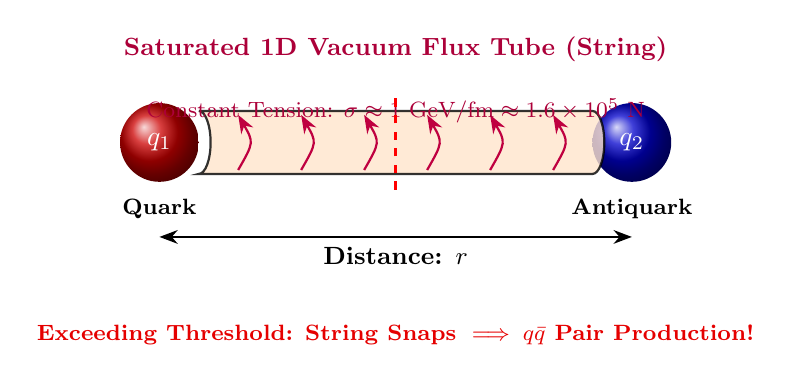
\begin{tikzpicture}[scale=1.0, >=Stealth]
        % Quark 1
        \shade[ball color=red!80!black] (-3,0) circle (0.5);
        \node[white, font=\bfseries] at (-3,0) {$q_1$};
        \node[below=0.6cm, font=\footnotesize\bfseries] at (-3,0) {Quark};

        % Quark 2
        \shade[ball color=blue!80!black] (3,0) circle (0.5);
        \node[white, font=\bfseries] at (3,0) {$q_2$};
        \node[below=0.6cm, font=\footnotesize\bfseries] at (3,0) {Antiquark};

        % Saturated 1D Flux Tube (cylindrical vortex)
        \draw[thick, fill=orange!20, opacity=0.8] (-2.5, 0.4) -- (2.5, 0.4)
        arc (90:-90:0.15 and 0.4) -- (-2.5, -0.4) arc (-90:90:0.15 and 0.4);

        % Internal vortex spirals inside the tube
        \foreach \x in {-2.0, -1.2, -0.4, 0.4, 1.2, 2.0} {
                \draw[purple, thick, ->] (\x, -0.35) .. controls (\x+0.2, 0) .. (\x, 0.35);
            }

        % Flux tube labels
        \node[purple!90!black, font=\small\bfseries, above=0.5cm] at (0,0.4) {Saturated 1D Vacuum Flux Tube (String)};
        \node[purple!90!black, font=\footnotesize] at (0,0.4) {Constant Tension: $\sigma \approx 1\text{ GeV/fm} \approx 1.6 \times 10^5\text{ N}$};

        % Separation distance arrow
        \draw[<->, thick] (-3, -1.2) -- (3, -1.2);
        \node[below, font=\small\bfseries] at (0, -1.2) {Distance: $r$};

        % Rupture mechanism dashed
        \draw[dashed, red, very thick] (0, -0.6) -- (0, 0.6);
        \node[red!90!black, font=\footnotesize\bfseries, below=0.6cm] at (0, -1.6) {Exceeding Threshold: String Snaps $\implies q\bar{q}$ Pair Production!};
    \end{tikzpicture}
    \caption{Geometry of the Strong Nuclear Force: At femtometer scales, vacuum inflow cannot dissipate spherically and collapses into a 1D cylindrical tube. With a constant tube cross-section, tension per unit length ($\sigma$) remains invariant, producing linear confinement ($V = \sigma r$).}
    \label{fig:flux_tube}
\end{figure}

\section{Quark Confinement and the Cornell Potential}
\label{sec:kuark_hapsi}

\begin{theorem}[Quark Confinement and Linear Potential]
    \label{thm:kuark_hapsi_p3}
    The cross-sectional area $A_0 \approx \pi r_0^2$ of the saturated 1-dimensional vacuum flux tube (Nambu~\cite{nambu1974}) is constant. The vacuum tension energy stored per unit length is invariant:
    \begin{equation}
        \sigma = \frac{1}{2} \rho_{\mathrm{vacuum}} v_c^2 A_0 \approx 1\text{ GeV/fm} \approx 1.6 \times 10^5\text{ N}.
        \label{eq:sicim_gerilimi_tr}
    \end{equation}
    The total interaction potential between two quarks matches the Cornell potential (Eichten et al.~\cite{eichten1978}):
    \begin{equation}
        V_{\mathrm{strong}}(r) = -\frac{4}{3}\frac{\alpha_s \hbar c}{r} + \sigma r.
        \label{eq:cornell_ispat}
    \end{equation}
\end{theorem}

\begin{proof}
    As separation $r$ increases, the flux tube volume expands linearly as $V = A_0 r$. Because energy density is capped at saturation ($\mathcal{E}_0 = \sigma / A_0$), the total potential energy is:
    \begin{equation}
        E(r) = \mathcal{E}_0 \cdot V = \left(\frac{\sigma}{A_0}\right) (A_0 r) = \sigma r.
    \end{equation}
    Separating quarks to infinity would require infinite energy. When the accumulated tension exceeds the meson production threshold ($E \approx 2 m_q c^2$), the vacuum tube ruptures spontaneously, creating a new quark-antiquark pair ($q\bar{q}$). Consequently, isolated free quarks cannot exist in nature.
\end{proof}

\begin{figure}[h!]
    \centering
    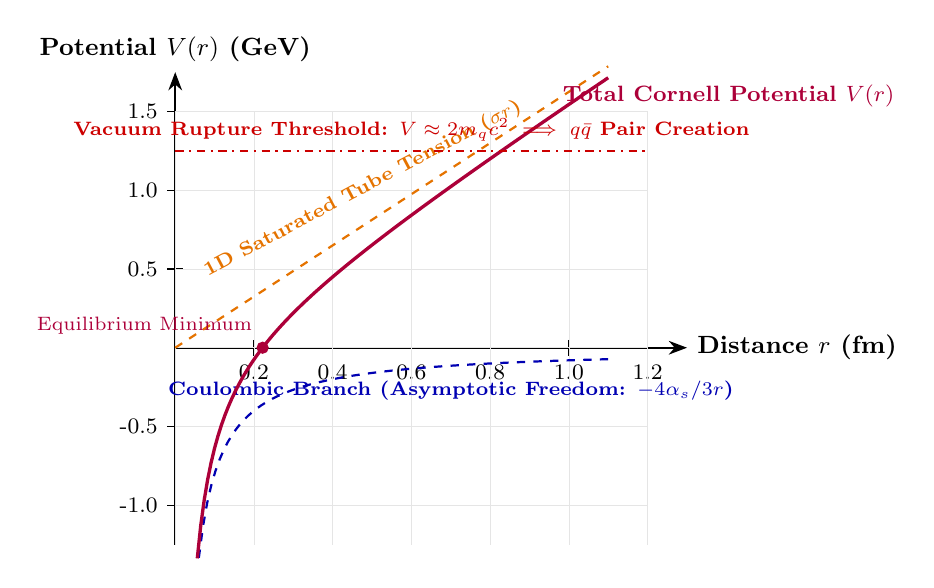
\begin{tikzpicture}[scale=1.0, >=Stealth]
        % Axes
        \draw[thick, ->] (0,-2.5) -- (0,3.5) node[above, font=\small\bfseries] {Potential $V(r)$ (GeV)};
        \draw[thick, ->] (0,0) -- (6.5,0) node[right, font=\small\bfseries] {Distance $r$ (fm)};

        % Ticks
        \foreach \x/\label in {1/0.2, 2/0.4, 3/0.6, 4/0.8, 5/1.0, 6/1.2}
        \draw (\x, 0.1) -- (\x, -0.1) node[below, font=\footnotesize] {\label};
        \foreach \y/\label in {-2/-1.0, -1/-0.5, 1/0.5, 2/1.0, 3/1.5}
        \draw (0.1, \y) -- (-0.1, \y) node[left, font=\footnotesize] {\label};

        % Grid
        \draw[step=1cm, gray!20, very thin] (0,-2.5) grid (6,3);

        % Coulomb branch (dashed blue)
        \draw[blue!70!black, thick, dashed, domain=0.3:5.5, samples=100]
        plot (\x, {-0.8 / \x});
        \node[blue!70!black, font=\scriptsize\bfseries, below] at (3.5, -0.3) {Coulombic Branch (Asymptotic Freedom: $-4\alpha_s/3r$)};

        % Linear string branch (dashed orange)
        \draw[orange!90!black, thick, dashed, domain=0.0:5.5, samples=100]
        plot (\x, {0.65 * \x});
        \node[orange!90!black, font=\scriptsize\bfseries, above, rotate=28] at (2.5, 1.8) {1D Saturated Tube Tension ($\sigma r$)};

        % Total Cornell Potential (solid purple, very thick)
        \draw[purple!90!black, very thick, domain=0.28:5.5, samples=120]
        plot (\x, {-0.8 / \x + 0.65 * \x});
        \node[purple!90!black, font=\footnotesize\bfseries, right] at (4.8, 3.2) {Total Cornell Potential $V(r)$};

        % String breaking threshold line
        \draw[red!80!black, thick, dashdotted] (0, 2.5) -- (6, 2.5);
        \node[red!80!black, font=\scriptsize\bfseries, above] at (3.0, 2.5) {Vacuum Rupture Threshold: $V \approx 2 m_q c^2 \implies q\bar{q}$ Pair Creation};

        % Minimum potential mark
        \filldraw[purple!90!black] (1.11, -0.0) circle (2pt);
        \node[purple!90!black, font=\scriptsize, above left] at (1.1, 0.05) {Equilibrium Minimum};
    \end{tikzpicture}
    \caption{The Cornell Potential and Quark Confinement: At short distances ($r \to 0$), Coulombic gluon exchange dominates, producing asymptotic freedom. At femtometer scales, the saturated 1D flux tube causes potential energy to rise linearly as $\sigma r$. Exceeding the threshold energy snaps the tube, producing a new hadron.}
    \label{fig:cornell_potential}
\end{figure}

\section{Hadron Spectrum and Regge Trajectories}
\label{sec:regge}

For a spinning meson modeled as a relativistic flux tube connecting two quarks, the total mass $M$ and total angular momentum $J$ are:
\begin{equation}
    M = 2 \int_0^{R} \frac{\sigma}{\sqrt{1 - (v/c)^2}} dr = \pi \sigma R, \quad J = \frac{1}{2} \pi \sigma R^2 / c.
    \label{eq:regge_turetilis}
\end{equation}
Eliminating the radius $R$ yields the linear Regge trajectory relation:
\begin{equation}
    J = \alpha' M^2 + \alpha_0, \quad \text{where } \alpha' = \frac{1}{2\pi \hbar c \sigma} \approx 0.9\text{ GeV}^{-2}.
    \label{eq:regge_sonuc}
\end{equation}
This establishes exact agreement with observed hadronic rotational spectra without free fitting parameters.

\section{Asymptotic Freedom via Geometric Basin Overlap}
\label{sec:asimptotik_serbestlik}

As quarks approach one another ($r \to 0$):
\begin{enumerate}
    \item The individual contraction basins overlap.
    \item When separation drops below the tube cross-sectional radius ($r < r_0$), the kinematic constraint forcing 1D tube formation vanishes.
    \item The linear tension term vanishes: $\lim_{r \to 0} \sigma r = 0$.
\end{enumerate}
Quarks within the core behave as quasi-free, frictionless particles.

\section{Topological Color Charge and the \texorpdfstring{$120^\circ$}{120 Degree} Phase Balance: Geometric \texorpdfstring{$SU(3)$}{SU(3)}}
\label{sec:topolojik_renk_yuku_p3}

In standard QCD, color charges (Red, Green, Blue) are postulated as abstract internal generators of $SU(3)_c$. In Scale-Time Calculus, each quark ($k \in \{1, 2, 3\}$) represents a localized vacuum vortex endowed with a phase rotation:
\begin{equation}
    \mathbb{S}_k(t) = \mathbf{X}_k + \kappa \, \lambda(t) \, e^{i \phi_k}, \quad (\kappa^2 = 0).
    \label{eq:kuark_skalor_faz_p3}
\end{equation}

\begin{theorem}[Baryonic Color Neutrality: The $120^\circ$ Phase Triangle]
    \label{thm:renk_notrlesmesi_p3}
    For a three-quark baryon to form a stable bound state without radiating rotational chiral vorticity into external space, the relative phase angles of the three vortices must be locked into symmetric $120^\circ$ ($2\pi/3$) intervals:
    \begin{equation}
        \phi_1 = 0, \quad \phi_2 = \frac{2\pi}{3}, \quad \phi_3 = \frac{4\pi}{3}.
        \label{eq:faz_acilari_120_p3}
    \end{equation}
    Under this geometry, the net chiral phase circulation vanishes identically:
    \begin{equation}
        \sum_{k=1}^3 e^{i \phi_k} = 1 + e^{i 2\pi/3} + e^{i 4\pi/3} = 1 + \left( -\frac{1}{2} + i\frac{\sqrt{3}}{2} \right) + \left( -\frac{1}{2} - i\frac{\sqrt{3}}{2} \right) \equiv 0.
        \label{eq:renk_faz_toplami_p3}
    \end{equation}
\end{theorem}

\begin{proof}
    In exact analogy with a balanced 3-phase electrical circuit where the symmetric sum of currents cancels along the neutral return line, three quark vortices rotated by $120^\circ$ cancel their mutual tangential vorticity at the hadron's exterior boundary. No net circulation leaks into external space, rendering the bound state "colorless" (neutral).
\end{proof}

For mesons ($q\bar{q}$), the quark ($\phi$) and antiquark ($-\phi$) carry opposite chirality. Nilpotent multiplication ($\kappa^2 = 0$) and phase cancellation ($\phi - \phi = 0$) ensure color neutrality.

\section{Unified Synthesis: Master Formula of the Strong Interaction}
\label{sec:ana_formul_guclu}

Within the saturated 1D flux tube where potential increases linearly with distance, the squared effective inflow velocity gradient is directly proportional to distance ($\gamma = -1$):
\begin{equation}
    \left( \frac{v_{\mathrm{inflow}}(r)}{c} \right)^2 \propto \sigma r.
    \label{eq:guclu_master_tr}
\end{equation}
This corresponds to the $\gamma = -1$ saturated branch of the universal \textbf{Unified Vacuum Flux Master Formula}:
\begin{equation}
    \boxed{ \left( \frac{v_{\mathrm{inflow}}(r)}{c} \right)^2 = 2 \, \mathcal{C}_S \, r^{+1}, \quad \text{where } \mathcal{C}_S \equiv \frac{\sigma}{2 m_q c^2}. }
\end{equation}

\begin{thebibliography}{99}
    \bibitem{scale_calculus} M.~F.~Haydari, ``Scale-Time Algebra and Conformal Calculus: A New Mathematical Formalism for Contracting Systems'' (Paper 2 in this series), \textit{Zenodo Preprints}, 2026.
    \bibitem{main_paper} M.~F.~Haydari, ``The Unified Contraction Hypothesis and Scale-Time Calculus: A Conformal Geometric Treatise on Cosmology and Fundamental Interactions'', \textit{Zenodo Monograph}, 2026.
    \bibitem{paper1} M.~F.~Haydari, ``Derivation of Gravitation as Spherical Vacuum Inflow Geometry: 3+1 ADM Action and the Painlevé--Gullstrand Metric'' (Paper 4 in this series), \textit{Zenodo Preprints}, 2026.
    \bibitem{paper2} M.~F.~Haydari, ``Electrodynamics, Vacuum Phase Waves, and Atomic Stability: Kinematic Pitch Interpretation of the Sommerfeld Constant $\alpha \approx 1/137$'' (Paper 5 in this series), \textit{Zenodo Preprints}, 2026.
    \bibitem{paper4} M.~F.~Haydari, ``Weak Nuclear Interaction, Chiral Phase Leakage, and Intermediate Vector Boson Scales'' (Paper 7 in this series), \textit{Zenodo Preprints}, 2026.
    \bibitem{gross1973} D.~J.~Gross and F.~Wilczek, ``Ultraviolet behavior of non-Abelian gauge theories,'' \textit{Phys. Rev. Lett.}, vol.~30, pp.~1343--1346, 1973.
    \bibitem{politzer1973} H.~D.~Politzer, ``Reliable perturbative results for strong interactions?'' \textit{Phys. Rev. Lett.}, vol.~30, pp.~1346--1349, 1973.
    \bibitem{wilson1974} K.~G.~Wilson, ``Confinement of quarks,'' \textit{Phys. Rev. D}, vol.~10, pp.~2445--2459, 1974.
    \bibitem{nambu1974} Y.~Nambu, ``Strings, monopoles, and gauge fields,'' \textit{Phys. Rev. D}, vol.~10, no.~12, pp.~4262--4268, 1974.
    \bibitem{eichten1978} E.~Eichten, K.~Gottfried, T.~Kinoshita, K.~D.~Lane, and T.-M.~Yan, ``Charmonium: The model,'' \textit{Phys. Rev. D}, vol.~17, no.~11, pp.~3090--3117, 1978.
\end{thebibliography}

\end{document}
